\setlength{\footskip}{8mm}

\chapter{Blob-Based Motion Analysis}
\label{ch:blobanalysis}

\textit{In this chapter, I review existing blob-based motion analysis
approaches including blob extraction, blob feature extraction, and
blob tracking. I provide details of our methods, and then I discuss
the feasibility of further improvement.}

\section{Introduction}

Motion analysis is the first key step in human behavior understanding,
since the results of later processes such as activity recognition rely
on the analysis.  Motion analysis provides a detailed synopsis of
object movement in the scene, on which foundation we can interpret the
activities in a surveillance video. This could save a tremendous
amount of human effort in monitoring or retrieving videos for review.

This dissertation focuses exclusively on blob-based motion analysis
methods. Our method assumes the camera is fixed relative to the scene
in which objects/people are moving.

\section{Literature Review}

In this section, I provide a review of existing methods for blob-based
motion analysis. The section is divided into three parts. The first
part is blob extraction, the second part is blob feature
extraction, and the last part is blob tracking.

\subsection{Blob Extraction}

Many approaches can be used to extract blobs or objects from a scene,
assuming the camera is fixed. The simplest approach is image
differencing. \shortciteA{yamato92hmm} use this method to extract
blobs representing humans in a scene based on the following
conditions:
\[
  \begin{array}{lc}
    {\rm if} & |{I_a (x,y) - I_b (x,y)}|< T,\;I_e (x,y) = 0 \\ 
    {\rm else} & I_e (x,y) = I_a (x,y).
  \end{array}
\]
$I_e (x,y)$ is the extracted human image, $I_a (x,y)$ is the original
image, $I_b (x,y)$ is a background image without any objects, and $T$
is a predefined threshold. This method can work well under specific
conditions but is not robust to noise, due to the use of a static
background image. In real-world situations, the background scene
changes over time.

\shortciteA{nair02surveillance} improve the image differencing 
technique by updating the background model and threshold over time for
every frame using temporal averaging. They first model the background
by taking the average of five consecutive frames without any object in
the scene. The labeled pixels are considered as foreground if they
satisfy the following condition:
\[
  |{I_n (x,y) - B_n (x,y)}| > T_n (x,y),
\]
where $I_n (x,y)$ is the current frame, $B_n (x,y)$ is the current
background model, and $T_n (x,y)$ is a threshold function. The authors
initialize the threshold value to 50 at all pixel locations. The
background model and threshold function are updated as follows:
\[
  \begin{array}{ll}
    B_{n + 1} (x,y) = \left\{ 
    \begin{array}{l}
      B_n (x,y) \\ 
      \alpha B_n (x,y) + (1 - \alpha )I_n (x,y) 
    \end{array} \right.
    &
    \begin{array}{l}
      {\rm if}\;(x,y)\;{\rm is}\;{\rm foreground}, \hfill  \\
      {\rm otherwise}, \hfill 
    \end{array}
  \end{array}
\]
\[
  \begin{array}{ll}
    T_{n + 1} (x,y) = \left\{
    \begin{array}{l}
      T_n (x,y) \\ 
      \alpha T_n (x,y) + 2(1 - \alpha)| {I_n (x,y) - B_n (x,y)}|
    \end{array} \right.
    &
    \begin{array}{l}
      {\rm if}\;(x,y)\;{\rm is}\;{\rm foreground}, \hfill  \\
      {\rm otherwise}, \hfill 
    \end{array}
  \end{array}
\]
where $\alpha$ is a constant to determine how fast $B_n (x,y)$ and
$T_n (x,y)$ adapt to changes. The update to $T_{n+1}(x, y)$ increases
the threshold when large variations in the background pixel
distribution are observed and decreases when little variation is
observed.

Although the image differencing technique is fast and commonly used in
many surveillance applications such as
ZoneMinder \shortcite{zoneminder}, a single model with a simple
threshold per pixel may not allow adaptation to multi-modal background
distributions.

Many researchers have attempted to improve background modeling to deal
with cluttered dynamic scenes. \shortciteA{wren97pfinder} model people
and the background scene separately using a single Gaussian
distribution per pixel in the YUV color space. Each pixel is
represented by a vector $[x, y, Y, U, V]^T$, where $(x, y)$ is the
pixel location and $(Y, U, V)$ is the color component. They classify
each pixel by calculating a likelihood for each class and selecting
the best one.  Based on the classification result, they update the new
model's parameters for each person and for the background scene
accordingly.  Using this background modeling technique with the proper
initial parameters yields reasonable results for both indoor and
outdoor scenes. Figure \ref{fig:car-sgm-result} shows sample results
for the single Gaussian background modeling method. Although this
technique can deal with noise, it is unsuitable for more cluttered
dynamic background scenes, especially outdoor scenes in which
multi-modal background distributions occur more frequently.

Several additional methods have been proposed to model backgrounds in
recent years. Examples include an eigenvalue decomposition-based
approach\shortcite{oliver00modeling}, a kernel density
estimation-based approach \shortcite{elgammal02background}, and a
median-based approach \shortcite{li06behavior}.

One of the best-known background modeling techniques is that
of \shortciteA{stauffer99background}, who propose a method that models
multi-modal background distributions using a mixture of Gaussian (MoG)
distributions. This technique works well in many cluttered dynamic
scenes. It also outperforms the single Gaussian background modeling
method outdoors, since multi-modal background distributions occur
frequently in outdoor scenes. The authors model the recent history of
each pixel using a mixture of $K$ Gaussian distributions. $K$ is
determined by the available memory and computational power. They
classify pixel values that do not fit one of the background
distributions as foreground until one of the Gaussian distributions
supports those values. Figure \ref{fig:car-mog-result} shows sample
results for the MoG background modeling method.

\begin{figure}[t]
  \centering
  \subfloat[]{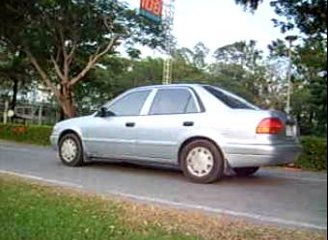
\includegraphics[scale=0.5]{figures/car-original.jpg}
  \label{fig:car-original}}
  \hspace{0.1in}
  \subfloat[]{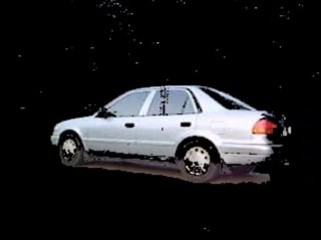
\includegraphics[scale=0.5]{figures/car-sgm-result.jpg}
  \label{fig:car-sgm-result}}
  \hspace{0.1in}
  \subfloat[]{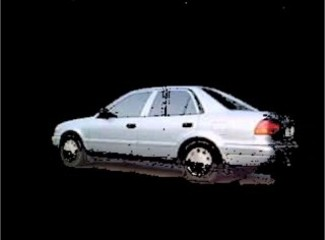
\includegraphics[scale=0.5]{figures/car-mog-result.jpg}
  \label{fig:car-mog-result}}
  \caption[Example results for single and MoG background modeling
    methods.]  {\small Example results for single and MoG background
    modeling methods. (a) Original image. (b) Foreground pixels using
    the single Gaussian background modeling method. (c) Foreground
    pixels using the MoG background modeling method. Reprinted from
    Tuan Anh (2008)\nocite{anh08thesis}.}
  \label{fig:bck-model-results}
\end{figure}

However, the MoG background modeling method faces problem \DIFdelbegin \DIFdel{ห }\DIFdelend dealing
with gradual illumination changes, as seen in
Figure \ref{fig:poppe-mog-result}. \shortciteA{poppe07background}
propose a new version of the MoG background modeling method to solve
this problem. The idea is to store the previous pixel value and
previous matching model number and use them in the matching step. In
the matching step, each pixel is checked against the $K$ Gaussian
distributions. For the model that matches the pixel in the previous
frame, if the difference between the current pixel value and previous
pixel value is smaller than a threshold, an intermediate match is
defined; otherwise, the normal matching step is followed. If the
matched model represents the background, the model number and the
current pixel value are stored; otherwise, they retain their
values. By doing this, foreground objects will not affect the recent
history. Figure \ref{fig:poppe-bck-model-results} shows example
results of using the MoG background modeling method and Poppe et al.'s
improved MoG background modeling method.

\begin{figure}[t]
  \centering
  \subfloat[]{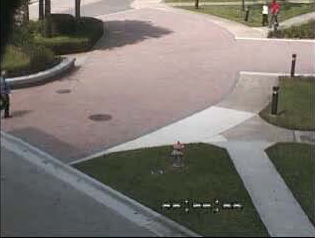
\includegraphics[scale=0.5]{figures/poppe-original.png}
  \label{fig:poppe-original}}
  \hspace{0.1in}
  \subfloat[]{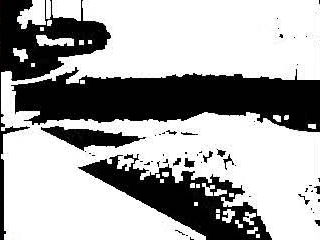
\includegraphics[scale=0.5]{figures/poppe-mog-result.png}
  \label{fig:poppe-mog-result}}
  \hspace{0.1in}
  \subfloat[]{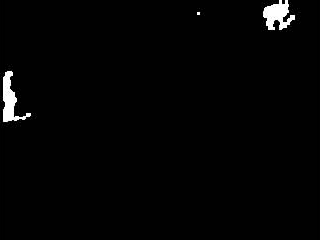
\includegraphics[scale=0.5]{figures/poppe-improved-mog-result.png}
  \label{fig:poppe-improved-mog-result}}
  \caption[Example MoG and improved MoG background modeling
    results.]{\small Example MoG and improved MoG background modeling
    results. (a) Original image. (b) Foreground pixels using MoG
    background modeling. (c) Foreground pixels using improved MoG
    background modeling. Reprinted from Poppe et al.\ (2007).}
  \label{fig:poppe-bck-model-results}
\end{figure}

Once the foreground is segmented from the background, moving blobs can
be extracted as connected components in the foreground mask.

\subsection{Blob Feature Extraction}

After segmenting blobs, we need to extract features to describe the
shape and dynamics of each blob. Extracted features are commonly used
in the blob tracking and behavior understanding processes.  In this
section, I review blob feature extraction methods used in existing
systems.

\shortciteA{yamato92hmm} extract mesh features from foreground
blobs. Mesh features are low-level image features that have also been
successfully applied to complex 2D patterns such as multi-font
characters \shortcite{umeda82font}. Each binarized image ($M \times N$
pixels) is divided into a mesh with $M_M \times N_M$ cells. They
represent each binarized image by a feature vector in which each
element is the proportion of black pixels in each
cell. Figure \ref{fig:mesh-feature} shows how mesh features are
calculated.

\begin{figure}[t]
  \centering
  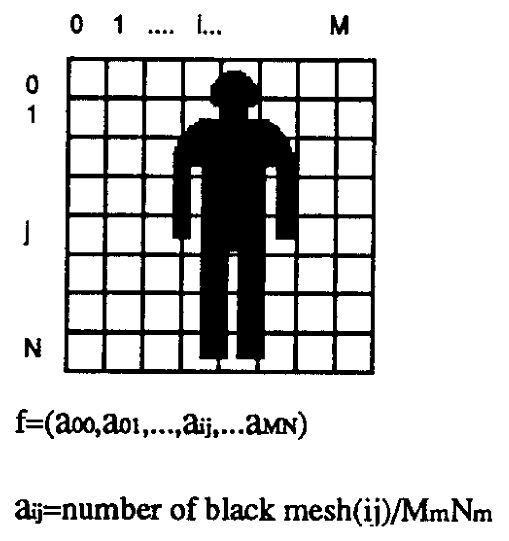
\includegraphics[width=2in]{figures/mesh-feature.jpg}  
  \caption[Mesh feature calculation.]{\small Mesh feature
    calculation. Reprinted from Yamato et al.\ (1992).}
  \label{fig:mesh-feature}
\end{figure}

\shortciteA{nair02surveillance} represent an extracted blob by a
feature vector that contains the coordinates of the blob's center of
mass, average color, and height. They use a $k$-means algorithm to
compute a set of codebook vectors from a set of feature vectors in the
training data. Once the $k$-means model is trained, they map a feature
vector to the index of the nearest codebook vector using Euclidean
distance. They then generate and output a sequence of codebook
vectors, which are then input to behavior modeling.

Star skeletonization is a technique that represents the gross
extremity structure of a blob. For humans, the gross extremities would
normally be the head, arms, and legs. \shortciteA{fujiyoshi98motion}
use this technique for analyzing human
motion. Figure \ref{fig:star-skeleton-example} shows an example of two
different star skeletons extracted from two human motions.

\begin{figure}[t]
  \centering
  \begin{tabular}{c}
    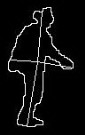
\includegraphics{figures/star-walking-01.jpg} 
    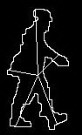
\includegraphics{figures/star-walking-02.jpg} 
    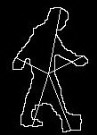
\includegraphics{figures/star-walking-03.jpg} 
    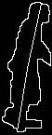
\includegraphics{figures/star-walking-04.jpg} \\
    (a) \\
    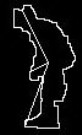
\includegraphics{figures/star-sit-01.jpg} 
    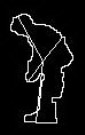
\includegraphics{figures/star-sit-02.jpg} 
    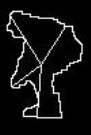
\includegraphics{figures/star-sit-03.jpg} 
    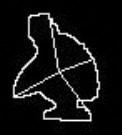
\includegraphics{figures/star-sit-04.jpg} \\
    (b)
  \end{tabular}
  \caption[Example star skeletons.]{\small Example star skeletons
    extracted from two human motions. (a) Walking. (b) Leaning forward
    and sitting down. Reprinted from Tuan Anh
    (2008)\nocite{anh08thesis}.}
  \label{fig:star-skeleton-example} 
\end{figure}

Some feature extraction methods have the ability to capture motion
history rather than only capturing current static features.  One such
method is space-time image features. \shortciteA{li06behavior} propose
a method based on space-time image features for automatic behavior
modeling and recognition. Their method is simple and insensitive to
noise, and it does not need to track parts of the human body. They
represent object shape using space-time images. After the foreground
is extracted, they equidistantly divide the bounded rectangle of the
foreground into $10\times7$ sub-blocks then normalize the value of
each sub-block as follows:
\[
  d_i = \left\lfloor {\frac{{s_i}}{{M}}\times255} \right\rfloor, i =
    1,2, \ldots,k,
\]
where $k=10\times7$ is the number of sub-blocks; $s_i$ is the number
of foreground pixels in the $i^{th}$ sub-block, and $M$ is the maximum
value of $s_i$, where $i=1,2,...,k$. The resulting shape descriptor
$D_t$ at image frame $t$ is defined as $D_t =
[d_1,d_2,d_3,...,d_k]$. To represent the motion of a sequence with $t$
frames, they construct the space-time image representation (see
Figure \ref{fig:space-time-feature}) as a matrix $I$ of size $t\times
k$:
\[
  I = [D_1,D_2,D_3, \ldots ,D_t]^{T}_{t\times k}
\]
They then extract the features from this representation by Gabor
filtering as follows:
\[
  F_n (x,y) = \iint {I_n (x_1 ,y_1 )G(x - x_1 ,y - y_1 ,f)dx_1dy_1},
\]
\[
  G(x,y,f) = \frac{1}{{2\pi \sigma _x \sigma _y }}\exp \left[ {
  - \frac{1}{2}\left( {\frac{{x^2 }}{{\sigma _x^2 }} + \frac{{y^2
  }}{{\sigma _y^2 }}} \right)} \right]M(x,y,f),
\]
\[
  M(x,y,f) = \cos \left[ {2\pi f(x\cos \theta +
  y\sin \theta)} \right],
\]
where $I_n(x,y)$ is the $n^{th}$ space-time image; $F_n(x,y)$ is the
filtered space-time image; the space constants of the Gaussian
envelope along the $x$ and $y$ axis are represented by $\delta _x$ and
$\delta _y$, respectively, and $f$ is the frequency of the sinusoid
and $\theta$ is the orientation of the Gabor filter.

\begin{figure}[t]
  \centering
  \begin{tabular}{cc}
    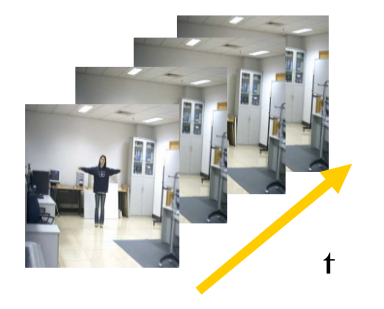
\includegraphics[width=2in]{figures/space-time-original.png} &
    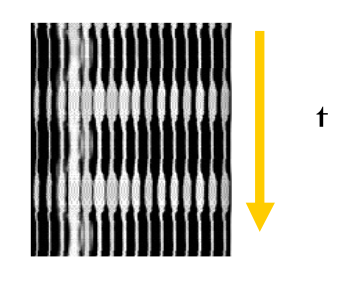
\includegraphics[width=2in]{figures/space-time-image.png} \\
    (a) & (b)
  \end{tabular}
  \caption[Space-time image representation.]{\small Space-time image
    representation. (a) Original video sequence. (b) Space-time image
    for the ``hand clapping'' behavior. Reprinted from H.\ Li et al.\
    (2006).}
  \label{fig:space-time-feature}
\end{figure}

Finally, H.\ Li et al.\ extract statistical features in each
$4 \times 5$ block of each short space-time image. The feature value
is the mean:
\[
  m = \frac{\displaystyle\sum_B | F_n(x, y)|}{K},
\]
where $B$ is a $4 \times 5$ block in the short space-time images, and
$K$ is the number of pixels in blob $B$. Each short space-time image
$V_i$, where $1 \le i \le N$, is represented as a $16 \times 14$
feature vector:
\[
  V_i = [M_1, M_2, \ldots, M_n, \ldots, M_{16}]^T,
\]
where $M_n = (m_{n1}, m_{n2}, \ldots, m_{ni}, \ldots, m_{n14})$.

\shortciteA{davis97mhi} propose a feature extraction method using
motion history image (MHI). MHI is a static image template where pixel
intensity is a function of the recency of motion in the video
sequence. The idea is to represent how the object is moving. The MHI
is defined as:
\[
  \begin{array}{ll}
    H_\tau (x,y,t) = \left\{ 
    \begin{array}{l}
      \tau \\ 
      \max (0, H_\tau (x, y, t - 1) - 1)
    \end{array} \right.
    &
    \begin{array}{l}
      {\rm if}\;D(x, y, t) = 1, \hfill  \\
      {\rm otherwise}, \hfill 
    \end{array}
  \end{array}
\]
where $H_\tau (x,y,t)$ represents the MHI for a pixel $(x,y)$ at time
$t$. The more recently moving pixels will be
brighter. Figure \ref{fig:mhi} presents example MHIs. The more
recently moving pixels are brighter.

\begin{figure}[t]
  \centering
  \begin{tabular}{ccc}
    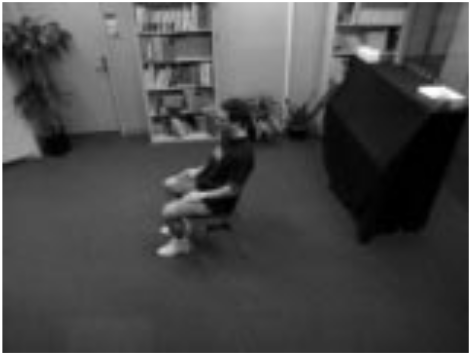
\includegraphics[width=1.5in]{figures/mhi-sit-original.png} &
    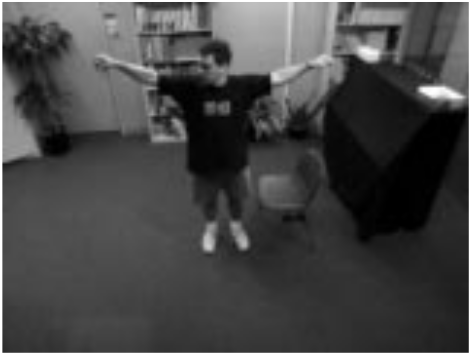
\includegraphics[width=1.5in]{figures/mhi-wave-original.png} &
    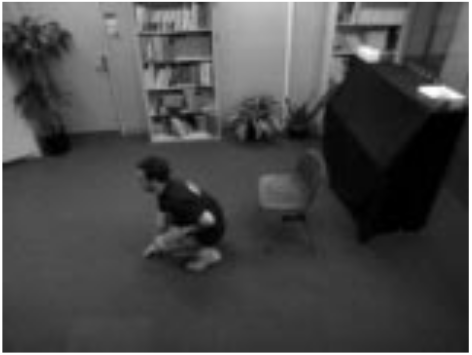
\includegraphics[width=1.5in]{figures/mhi-crouch-original.png} \\
    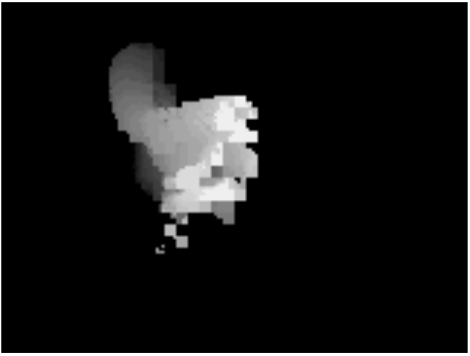
\includegraphics[width=1.5in]{figures/mhi-sit-results.png} &
    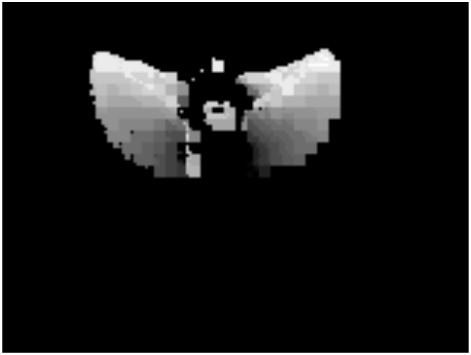
\includegraphics[width=1.5in]{figures/mhi-wave-results.png} &
    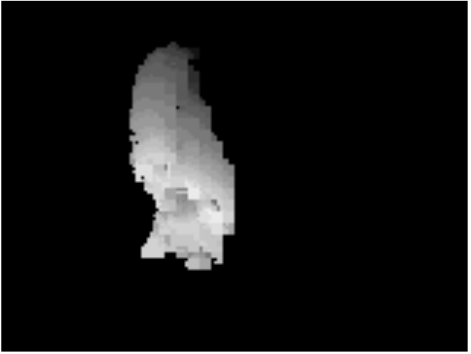
\includegraphics[width=1.5in]{figures/mhi-crouch-results.png} \\
    sit-down & arms-wave & crouch-down 
  \end{tabular}
  \caption[Example motions along with their motion history images
    (MHIs).]{\small Example motions along with their motion history
    images (MHIs). Reprinted from J.\ W.\ Davis and Bobick (1997).}
  \label{fig:mhi}
\end{figure}

Based on the local intensity history of
pixels, \shortciteA{xiang02event} propose a new low-level primitive
applicable to human representation that can describe human actions
efficiently, namely, the pixel change history (PCH).  The PCH is
capable of characterizing pixel-wise temporal visual information in
order to detect pixel-level events. It is a representation of
pixel-wise changes based on a combination of the pixel signal energy
(PSE) proposed by \shortciteA{ng03pixel} and the MHI. The PCH is
computed as follows:
\[
  P_{\varsigma ,\tau } (x,y,t) = \left\{ \begin{array}{l}
  \min (P_{\varsigma ,\tau } (x,y,t - 1) + \frac{{255}}{\varsigma },255)\quad 
  \; {\rm if}\;D(x,y,t) = 1 \\ 
  \max (P_{\varsigma ,\tau } (x,y,t - 1) + \frac{{255}}{\tau },0)\quad \quad 
  {\rm otherwise}, \\ 
  \end{array} \right.
\]
where $P_{\varsigma ,\tau } (x,y,t)$ represents the PCH for a pixel
$(x,y)$ at time $t$, $D(x,y,t)$ indicates foreground regions at time
$t$, $\varsigma$ is an accumulation factor, and $\tau$ is a decay
factor. When the accumulation factor is set to 1, the PCH over the
entire image is equivalent to the MHI. 

\shortciteA{xiang08incremental} use a discrete scene-wide event-based
approach for behavior pattern representation. This approach is
effective for cluttered scenes compared to the trajectory-based
representations used in most existing approaches. Xiang and Gong model
the foreground pixels using PCH \shortcite{xiang02event}, group them
into blobs, and define a scene event if the average PCH value of a blob is
larger than a defined threshold. They then represent a scene event as
a 7-dimensional feature vector
\[
  \vec{f} = [ \bar{x}, \bar{y} , w, h, R_f , M_px, M_py],
\]
where $(\bar{x}, \bar{y})$ is the centroid of the blob, $w$ and $h$
are the width and height of the bounding box associated with the blob,
respectively, $R_f$ is the filling ratio of foreground pixels within
the bounding box, and $(M_px, M_py)$ are a pair of first order moments
of the PCH image within the bounding box. 

Recursive filtering \shortcite{masoud03recognition} is a technique
that encodes motion information such as the speed of the motion within
a short period of time. The idea is to represent the ``recency'' of
the motion. This technique is conceptually similar to the MHI. Let
$I_t$ be the frame at time $t$. The filtered image $F_t$ at time $t$
is defined as follows:
\[
  F_t = \left| {I_t  - M_t } \right|
\]
\[
  M_t = (1 - \beta)M_{t - 1}  + \beta M_t 
\]
\[
  M_0 = I_0 = {\rm Background},
\]
where $t = 1, 2, \cdots, n_i$. If $\beta = 0$, the filtered image
$F_t$ will be the foreground and if $\beta = 1$, $F_t$ will be
equivalent to image differencing. Examples of filtered images are
presented in Figure \ref{fig:f-img}.

\begin{figure}[t]
  \centering
  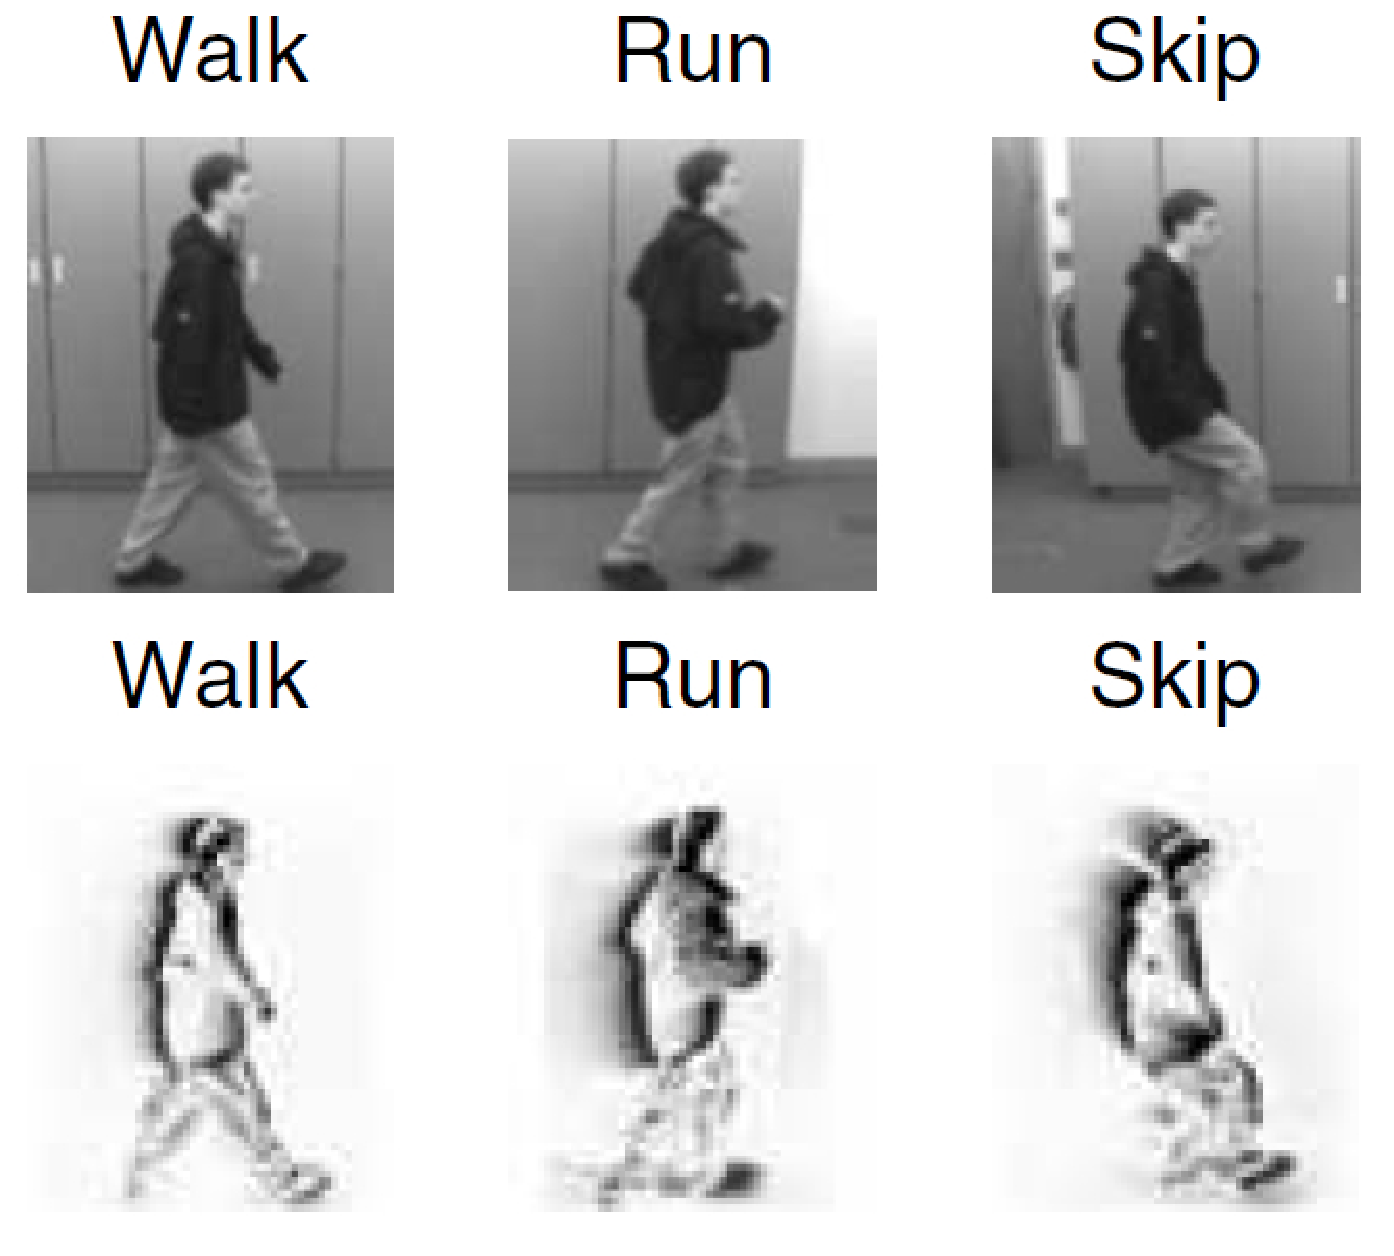
\includegraphics[width=2.5in]{figures/f-img}
  \caption[Example filtered images.]{\small Example filtered
    images. The coefficient $\beta$ is set to 0.5. Reprinted from
    Masoud and Papanikolopoulos (2003).}
  \label{fig:f-img}
\end{figure}

I describe the blob feature representation used in this dissertation
in Section \ref{sec:blob-appearance-based-blob-tracking}.

\subsection{Blob Tracking}

Tracking is one of the most active research areas in computer
vision. It can be used in a variety of applications, e.g.\ video
indexing, sports video enhancement, and visual surveillance.  In the
area of tracking, occlusion ambiguity is the most fundamental
difficulty.  It makes associating blobs with individuals or moving
objects that are partially or fully occluded in different frames
highly challenging, especially in complex scenes.

In video surveillance applications, person/object tracking is a
critical step prior to behavior modeling. Extracted information such
as the motion trajectory can be used to better understand activities
occurring in a scene.

The Kalman filter \shortcite{kalman60filtering} is a well-known
algorithm that has been extensively applied to tracking in many
domains.  In visual surveillance, \shortciteA{rosales99tracking}
propose a method for tracking multiple people in a 3D space. They
assume that the system uses a single uncalibrated video camera to
observe multiple moving people. They use an extended Kalman filter
(EKF) to estimate relative 3D motion trajectories up to a scale
factor.  They select only two feature points, the two opposite corners
of the person's bounding box, to reduce the complexity of the tracking
problem. The 3D size of the person's bounding box is assumed to remain
approximately the same or at least vary smoothly. People are
considered as plane objects, so the depth at both feature points
should be the same. The state vector then becomes:
\[
  \vec{x} = (x_0 ,y_0 ,x_1 ,y_1 ,z\beta ,\dot x_0 ,\dot y_0
  ,\dot x_1 ,\dot y_1 ,\dot z\beta )^T,
\]
where $(x_0, y_0, z\beta)^T$ and $(x_1, y_1, z\beta)^T$ are the
corners of the 3D planar bounding box, and $(\dot x, \dot y, \dot
z\beta)^T$ represents a corner's 3D velocity relative to the
camera. The experimental results demonstrate that Rosales and
Sclaroff's 3D trajectory-based estimation method significantly
improves the robustness over 2D trajectory-based estimation methods.
Figure \ref{fig:rosales-tracking-result} shows an example of 3D
tracking results for this method.

\begin{figure}[t]
  \centering
  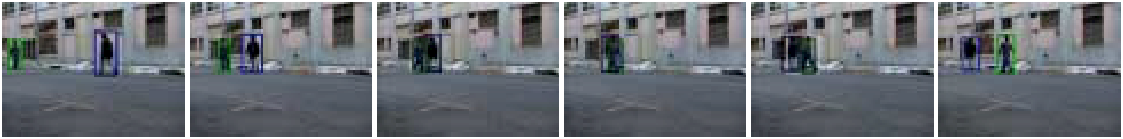
\includegraphics[width=6in]{figures/rosales-tracking-result.png}
  \caption[Sample 3D tracking results from Rosales and Sclaroff's
    method.]{\small Sample 3D tracking results from Rosales and
    Sclaroff's method. Two people walking along different trajectories
    then occluding each other. Reprinted from Rosales and Sclaroff
    (1999).}
  \label{fig:rosales-tracking-result}
\end{figure}

\shortciteA{bodor03recognition} develop an automated system to track
the positions of individual pedestrians using a Kalman filter and
alert security personnel when a pedestrian enters a secure area.

\shortciteA{niu03tracking} propose a method using a second-order
Kalman filter to track each person individually and handle occlusion
problems. They define a state that includes position, velocity, and
acceleration. When a new person is detected, they store a unique label
for that person having the information: height, centroid, and the
average intensity value of the region of the person. They then use
this information to continue keeping track of the person in each
frame.

\shortciteA{girondel04tracking} propose a multiple human tracking
method using the Kalman filter. They define a Kalman filter for each
person then predict the person's bounding box, the person's face's
bounding box, and the speed. They use a state vector of ten components
for each Kalman filter: the corners of the bounding boxes of the
person and face plus two components for face speed. They use skin
detection to detect face and hands and assume that face is a bigger
blob that moves more steadily. In this paper, they use the combination
of a forward tracking phase and a backward tracking phase to track
between detected objects on two consecutive frames. This technique is
also called ``forward and backward overlapping.'' I hereinafter
describe this technique in more details in
Section \ref{sec:blob-appearance-based-blob-tracking}.
Figure \ref{fig:girondel-tracking-result} shows an example of the
tracking results from Girondel et al.'s method.

\begin{figure}[t]
  \centering
  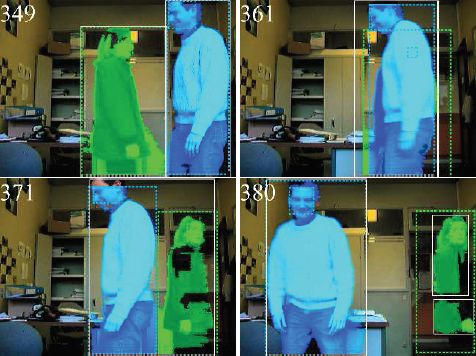
\includegraphics[width=2in]{figures/girondel-tracking-result.png}
  \caption[Sample tracking results from Girondel et al.'s
    method.]{\small Sample tracking results from Girondel et al.'s
    method. Reprinted from Girondel et al.\ (2004).}
  \label{fig:girondel-tracking-result}
\end{figure}

\shortciteA{lv06leftluggage} use a Kalman filter to track moving
blobs. The authors use a color histogram as an appearance model to
resolve the identity problem of blob merging. If the blob in the
current frame matches with multiple existing tracks, they use the
color histogram of each matched track to find the best-corresponding
blob. Figure \ref{fig:lv-blob-tracking-results} shows an example of
blob tracking results from Lv et al.'s method.  Color histograms are a
simple and efficient method that can be used to compare the similarity
of images. However, they lack spatial information. For instance, the
color histogram of an image with single large block of red pixels will
be similar to that of the image with same number of scattered red
pixels.

\begin{figure}[t]
  \centering
  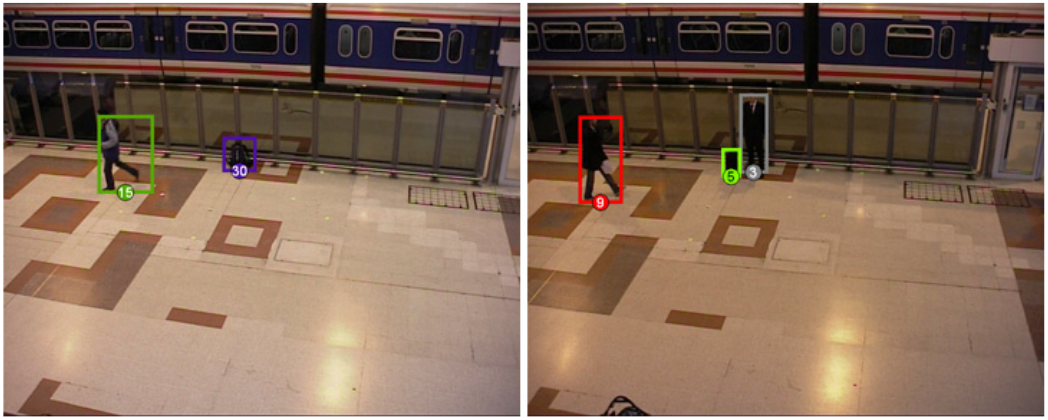
\includegraphics[width=4in]{figures/lv-blob-tracking-results.png}
  \caption[Sample tracking results from Lv et al.'s method.]{\small
    Sample tracking results from Lv et al.'s method. Reprinted from Lv
    et al.\ (2006).}
  \label{fig:lv-blob-tracking-results}
\end{figure}

\shortciteA{senior06tracking} solve occlusion problems by
modeling moving objects using an appearance model. They use an
appearance model to localize objects during partial occlusion, detect
complete occlusions and resolve depth ordering of objects during
occlusions. In this paper, they use a RGB color model as an appearance
model with an associated probability mask for each foreground
blob. The probability mask records the likelihood of the object being
observed at that pixel.  The appearance model of each blob is then
updated on subsequent frames. They also construct a distance matrix by
a bounding box distance measure. Then they use it to determine the
association between tracks and foreground blobs. This technique is
similar to the forward and backward overlap method. In this paper,
they evaluated the proposed method on the PETS 2001 data set, and the
results show that their algorithm successfully deals with complex
real-world interactions. Figure \ref{fig:senior-tracking-results}
shows an example of the tracking results from Senior et al.'s method.

\begin{figure}[t]
  \centering
  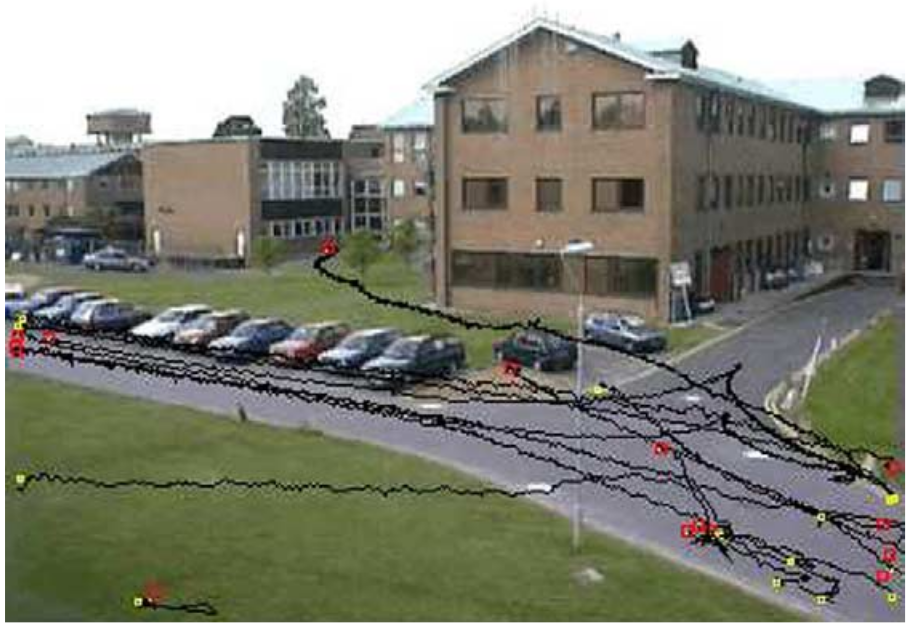
\includegraphics[width=3in]{figures/senior-tracking-results-for-dataset-1.png}
  \caption[Sample tracking results from Senior et al.'s
    method.]{\small Sample tracking results from Senior et al.'s
    method. Reprinted from Senior et al.\ (2006).}
  \label{fig:senior-tracking-results}
\end{figure}

In the following sections, I provide details of our blob-based motion
analysis including global motion detection in
Section \ref{sec:blob-motion-detection}, blob extraction in
Section \ref{sec:blob-blob-extraction}, appearance-based blob tracking
in Section \ref{sec:blob-appearance-based-blob-tracking}, and blob
feature vector discretization in
Section \ref{sec:blob-discretization}. I then finally discuss the
limitations and possible feasibilities for improving our method.

\section{Global Motion Detection}
\label{sec:blob-motion-detection}

Any video frames in which no motion occurs are removed to decrease
processing and storage time. We use simple frame-by-frame
subtraction. When the difference image has a number of pixels whose
intensity differences are above a threshold, we start a new video
segment. We use a threshold large enough not to trigger event
processing in a static scene, e.g.\ when a breeze makes leaves of a
tree move. We also buffer the no-motion frames for a period of time
and include some number of frames before and after the motion in the
event. This method avoids oversegmentation of events when moving
objects stop moving briefly.  In all of the experiments reported in
this dissertation, we start a new video segment when the number of
changed pixels in the 320$\times$240 input exceeds 300.

\DIFaddbegin \DIFadd{Through some preliminary empirical experimentation I found that 300 was a good 
threshold. While this simple approach worked well in our experimental setup, 
it would not work as well in a situation where the camera is subject to 
vibration, causing a large number of pixels to change values significantly.
}

\DIFaddend \section{Blob Extraction}
\label{sec:blob-blob-extraction}

After discarding the no-motion video segments, we use Poppe et al.'s
(2007) background modeling technique\nocite{poppe07background} to
segment foreground pixels from the background. As previously
mentioned, Poppe et al.\ extend the standard mixture of Gaussians
background model
\shortcite{stauffer99background} to handle gradual illumination changes.

\section{Appearance-Based Blob Tracking}
\label{sec:blob-appearance-based-blob-tracking}

\renewcommand{\algorithmicrequire}{\textbf{Input:}}
\renewcommand{\algorithmicensure}{\textbf{Output:}}
\renewcommand{\algorithmicforall}{\textbf{for each}}
\begin{algorithm}
\caption{Appearance-Based Blob Tracking}
\label{blob-tracking-algorithm}
\begin{algorithmic}
  \REQUIRE $B$: set of all current blobs
  \REQUIRE $T$: set of all current tracks
  \REQUIRE $M$: merged track association matrix
  \ENSURE $\widetilde{T}$: set of all revised tracks
  \ENSURE $\widetilde{M}$: revised merged track association matrix
  \STATE $\widetilde{T} \gets \emptyset$; $\widetilde{M} \gets \emptyset$; $L \gets \emptyset$
%  \STATE \COMMENT{Construct an overlap area matrix between the bounding box of blobs and tracks.}
  \STATE $A \gets \textsc{Get-Overlap-Area-Matrix}(B, T)$
  \FORALL{$t \in T$}
    \STATE \textbf{if} $t$ is marked as processed \textbf{then} continue
    \STATE $B' \gets \{ b' \mid A(b', t) > 0 \}$ \COMMENT{$B'$ contains candidate blobs for track $t$.}
    \STATE $T' \gets \{ t \} \cup \{ t' \mid M(t, t') = 1 \}$ \COMMENT{$T'$ contains all tracks currently merged with $t$.}
    \IF{$|B'| \geq 1$}
      \FORALL{$t' \in T'$}
        \STATE Let $b = \displaystyle\argmax_{b' \in B'} S(b', t')$
	\STATE $L \gets L \cup \{ (t', b) \}$
        %\STATE $\widetilde{t} \gets \textsc{Update-Track-Information}(t')$
        %\STATE $\widetilde{T} \gets \widetilde{T} \cup \{ \widetilde{t} \}$
	\STATE $\textsc{Mark-Track-As-Processed}(t')$
      \ENDFOR
%      \STATE Not needed ----- We may need it in case a blob reappears..
%    \ELSE
%      \FORALL{$t' \in T'$}
%         \STATE $s \gets \textsc{Get-Stale-Count}(t')$
%         \IF{$s > \theta_s$}
%           \STATE $\textsc{Mark-Track-For-Deletion}(t')$
%         \ENDIF
%      \ENDFOR
%      \STATE Not needed -----
    \ENDIF
  \ENDFOR
  \FORALL{$(t_i, t_j) \in T \times T$}
    %\STATE \COMMENT{If track $t_i$ links to the same blob $b$ as track $t_j$}
    \STATE If $\exists b$ s.t.\ $(t_i, b) \in L \wedge (t_j, b) \in L, \widetilde{M}_{ij} \gets 1$, otherwise $\widetilde{M}_{ij} \gets 0$
  \ENDFOR
  \STATE $T^* \gets \{ t^* \mid \neg\exists b \in B \;\text{s.t.}\; (t^*,b) \in L \}$ \COMMENT{$T^*$ contains tracks for which ``stale count'' will be increased.}
  \STATE $\widetilde{T} \gets \textsc{Update-Or-Delete-Stale-Tracks}(T,T^*)$
  \STATE $B^* \gets \{ b^* \mid \neg \exists t \in T \;\text{s.t.}\; (t, b^*) \in L \}$ \COMMENT{$B^*$ contains blobs with no tracks assigned.}
  \STATE $\widetilde{T} \gets\textsc{Add-New-Tracks-For-Not-Linked-Blobs}(\widetilde{T},B^*)$
\end{algorithmic}
\end{algorithm}

In this step, we take at time $t$ a list of blobs detected by the
previous step, a set of tracks updated at time $t-1$, and a merged
track association matrix.  We output an updated track list and merged
track association matrix.  Algorithm \ref{blob-tracking-algorithm} is
a pseudocode summary of our approach.  We first construct a matrix in
which each element indicates the overlap area of the bounding box of a
current blob with an existing track.  When a blob is found to
correspond to a single unique track, the track update is simple; we
just associate the blob with the track.  If a track is no longer
visible for some period of time, it will be considered \textit{stale}
and deleted. Special handling is required for cases in which a new
blob overlaps multiple old tracks (\textit{merges}) or multiple new
blobs overlap the same old track (\textit{splits}). To handle these
cases, our method evaluates a similarity function $S(b, t)$ for each
candidate blob-track pair $(b,t)$. $S(b,t)$ is based on the color
coherence vector (CCV; Pass et al., 1996)\nocite{pass96ccv}; when
tracks merge, we group them, but keep their identities separate, and
when tracks split, we associate the new blobs with the correct tracks
or groups of tracks by comparing their CCVs, on the assumption that
when an object eventually separates from the group, its appearance
will be similar to its appearance before the merge.  Our tracking
method performs very well on typical simple cases such as those shown
in Figure \ref{fig:normal-tracking-results} involving clear
trajectories of each moving person or object. However, it still has
some problems with more complex cases such as those shown in
Figure \ref{fig:complex-tracking-results} involving large groups of
people or objects moving together and interacting for some period of
time.

\begin{figure}[t]
  \begin{center}
    \begin{tabular}{ccccc}
      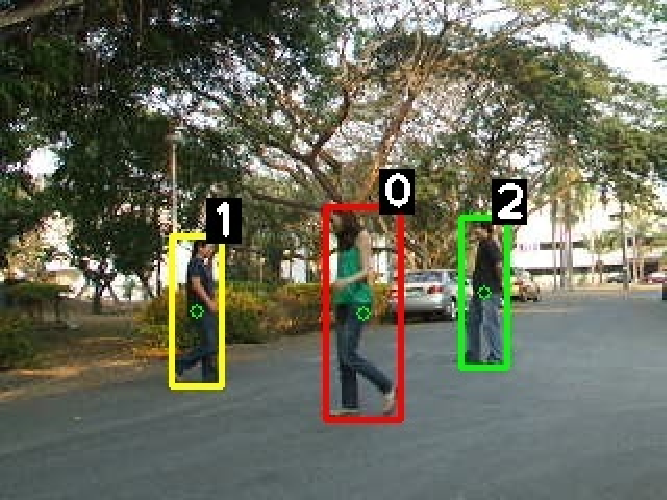
\includegraphics[scale=0.21]{figures/normal-tracking-result-0090.pdf} &
      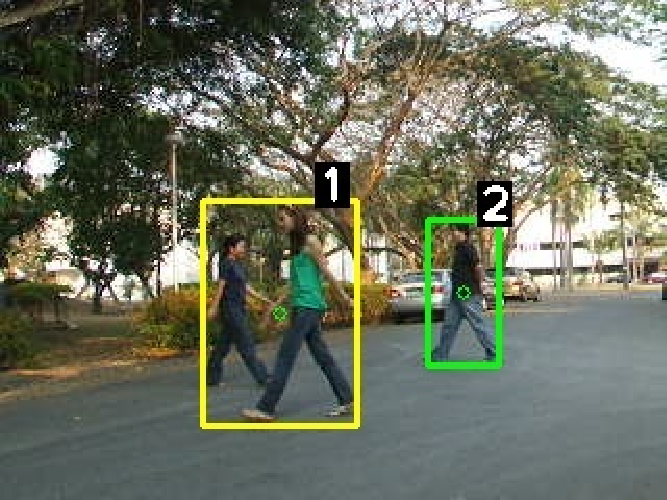
\includegraphics[scale=0.21]{figures/normal-tracking-result-0094.pdf} &
      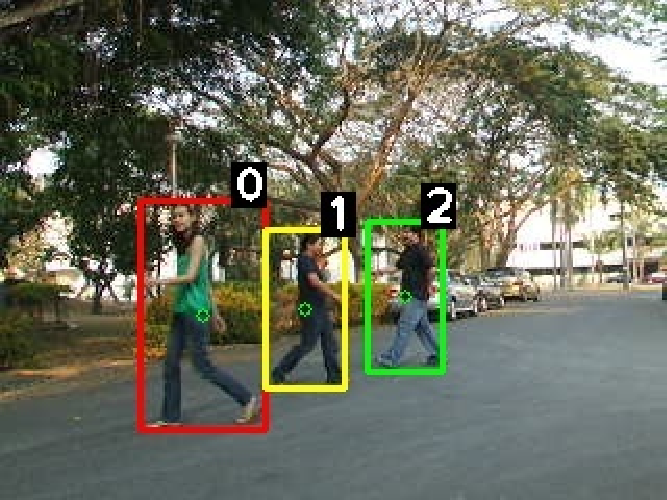
\includegraphics[scale=0.21]{figures/normal-tracking-result-0103.pdf} &
      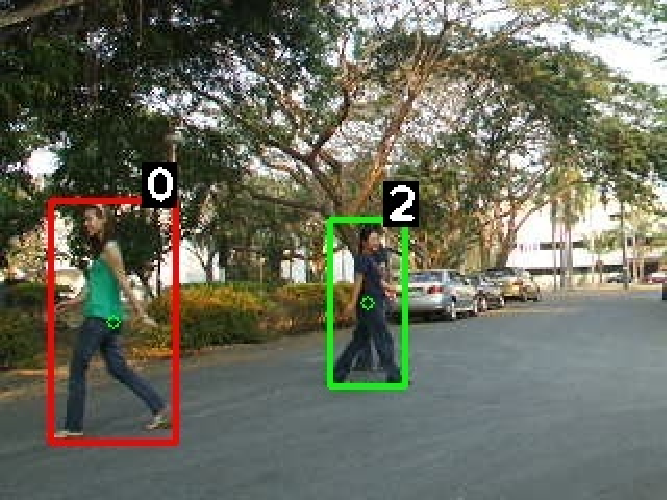
\includegraphics[scale=0.21]{figures/normal-tracking-result-0110.pdf} &
      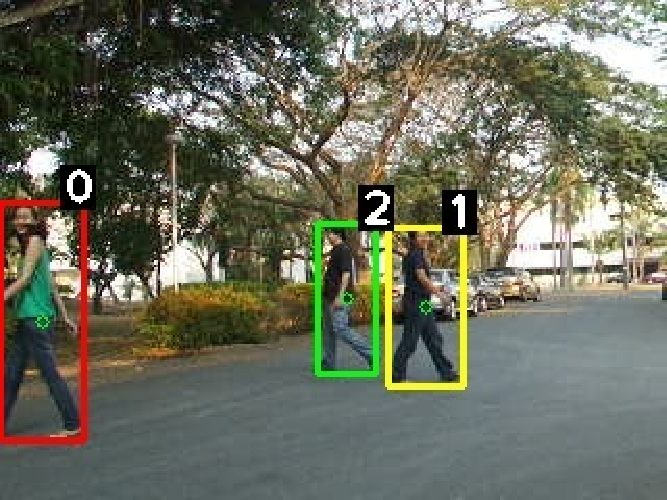
\includegraphics[scale=0.21]{figures/normal-tracking-result-0116.pdf} 
      \\
      \small Frame 90 & 
      \small Frame 94 & 
      \small Frame 103 & 
      \small Frame 110 & 
      \small Frame 116
    \end{tabular}
  \end{center}
  \caption[Sample blob tracking results for typical simple
    cases]{\small Sample blob tracking results for typical simple
    cases. In frame 94, track 0 and track 1 have merged.  In frame
    103, our method has correctly associated each motion blob with the
    correct track after they split. Similarly, frame 110 shows the
    result of another merge, and frame 116 shows the (correct) result
    when the merged motion blob splits.}
  \label{fig:normal-tracking-results}
\end{figure}

\begin{figure}[t]
  \begin{center}
    \begin{tabular}{ccccc}
      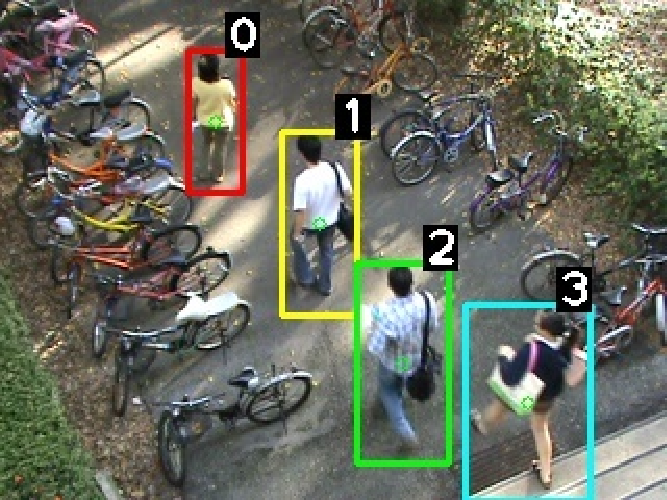
\includegraphics[scale=0.21]{figures/complex-tracking-result-0125.pdf} &
      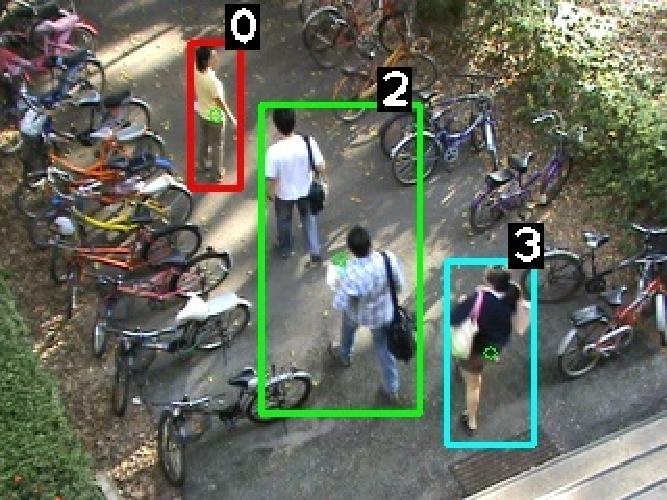
\includegraphics[scale=0.21]{figures/complex-tracking-result-0131.pdf} &
      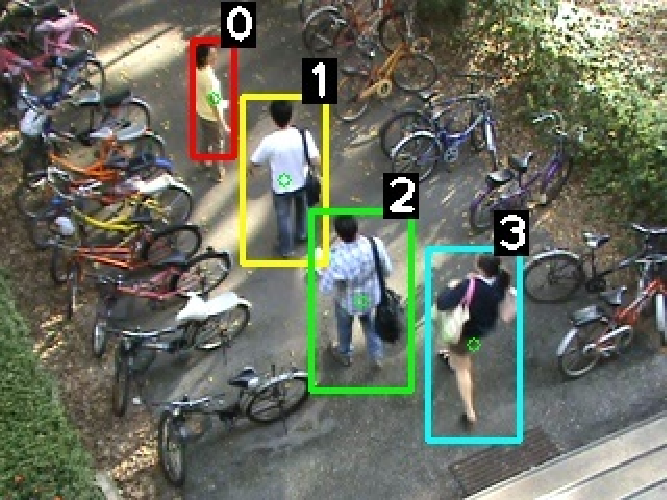
\includegraphics[scale=0.21]{figures/complex-tracking-result-0133.pdf} &
      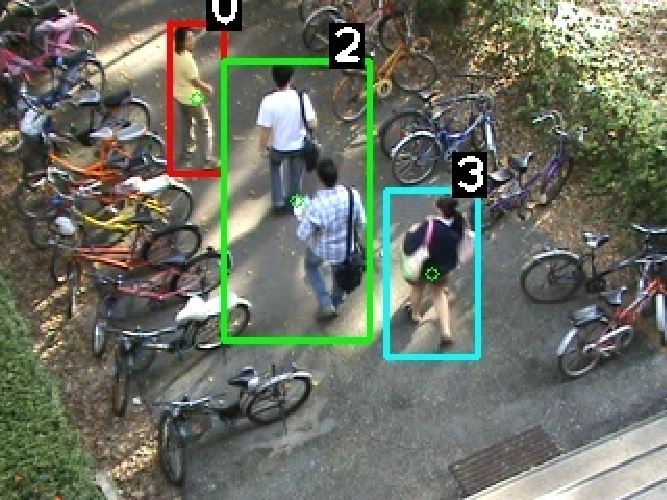
\includegraphics[scale=0.21]{figures/complex-tracking-result-0141.pdf} &
      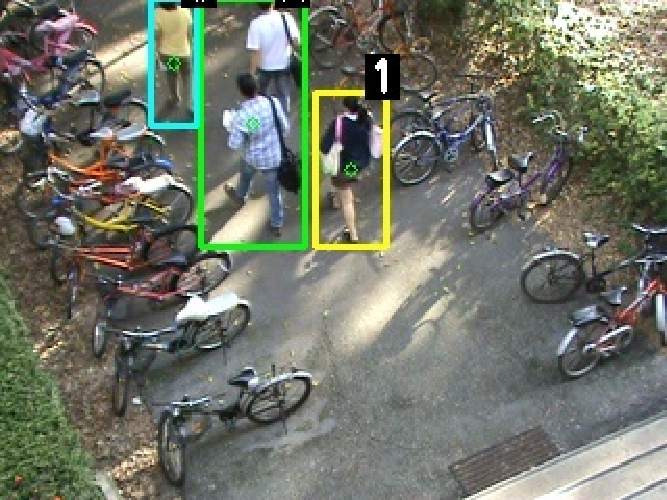
\includegraphics[scale=0.21]{figures/complex-tracking-result-0160.pdf} 
      \\
      \small Frame 125 & 
      \small Frame 131 & 
      \small Frame 133 & 
      \small Frame 141 & 
      \small Frame 160
    \end{tabular}
  \end{center}
  \caption[Sample blob tracking results for a complex case.]{\small
    Sample blob tracking results for a complex case. In frame 131,
    track 1 and track 2 have merged. In frame 133, our method has
    correctly associated the current motion blobs with tracks after
    the merged blob splits. However, when the merged blob shown in
    frame 141 splits (in frame 160), we observe a track ID switch
    error in associating blobs with tracks.}
  \label{fig:complex-tracking-results}
\end{figure}

Once the blob-to-track association is performed, we represent each
track $i$ at time $t$ by a feature vector
\[
    \vec{f}_i^t = \begin{bmatrix} x_i^t & y_i^t & s_i^t & r_i^t &
        dx_i^t & dy_i^t & v_i^t \end{bmatrix},
\]
where $(x_i^t, y_i^t)$ is the centroid of the blob associated with
track $i$. $s_i^t$ is the area, in pixels, of the detected
blob. $r_i^t$ is the aspect ratio of the blob's bounding box,
calculated by dividing the width of the bounding box by its height.
$(dx_i^t, dy_i^t)$ is the unit motion vector for the blob associated
with track $i$ at time $t$ compared to track $i$ at time
$t-1$. $v_i^t$ is a temporally smoothed version of the speed of the
blob associated with track $i$, calculated as
\[
    v_i^t = r \frac{{\sqrt {(x_i^t - x_i^{t - 1} )^2 + (y_i^t - y_i^{t -
        1} )^2 } }}{{\Delta t}} + (1 - r) v_i^{t-1},
\]
where $r$ is a constant (we use $r=0.5$ in our experiments), $\Delta
t$ is the capture time difference between the frames at time $t$ and
$t-1$.

A preliminary report on the results for this appearance-based blob
tracking method appeared in \shortciteA{shashi10thesis}. \DIFdelbegin \DIFdel{The previous
}\DIFdelend \DIFaddbegin \DIFadd{I worked with
Gharti to produce the initial version of the method.  Since the
initial }\DIFaddend implementation was simplistic in some cases \DIFdelbegin \DIFdel{, }\DIFdelend and some work was
redundant\DIFdelbegin \DIFdel{. In the current work, I have }\DIFdelend \DIFaddbegin \DIFadd{, I }\DIFaddend improved the code to get better blob matching\DIFdelbegin \DIFdel{and }\DIFdelend \DIFaddbegin \DIFadd{.  
In particular, the current implementation does not need to create and 
label each group of merged tracks but use only the information gained 
from the merged track association matrix. I also }\DIFaddend eliminated unnecessary 
cases in the blob-to-track association process.

\DIFdelbegin \DIFdel{Although }\DIFdelend Kalman filtering or other methods may be more optimal for
filtering blob position and velocity over time, \DIFaddbegin \DIFadd{and tracking blobs 
with the filters could indeed improve the tracking results. 
In this dissertation, }\DIFaddend we find that they are unnecessary in 
practice because we observe relatively little noise in our \DIFdelbegin \DIFdel{data}\DIFdelend \DIFaddbegin \DIFadd{blob 
position from the tracker}\DIFaddend , and we map the feature vectors to discrete 
symbols fairly coarsely in the next step.

\section{Blob Feature Vector Discretization}
\label{sec:blob-discretization}

For simplicity, we use discrete-observation hidden Markov models (HMMs) 
in this dissertation. This means that each feature vector $\vec{f}_i^t$ must
be mapped to a discrete category (cluster ID) in the set $V = \{ v_1,
v_2, \ldots, v_U \}$, where $U$ is the number of categories. We use
$k$-means clustering based on a training set to map feature vectors to
discrete clusters.  Prior to clustering, we normalize each feature by
a $z$-score \DIFaddbegin \DIFadd{as in \ref{eq:z-score}.  
}\begin{equation}\DIFadd{
    \label{eq:z-score}
    z = \frac{x - \mu}{\sigma}
}\end{equation}
\DIFadd{where $\mu$ is the mean and $\sigma$ is the standard deviation of each 
feature}\DIFaddend . The scale factors are independent for all features
except $x_i^t$ and $y_i^t$, for which we apply a single isotropic
scale factor.

In the training stage, we run $k$-means with $U$ cluster centers then
save the cluster centers as a codebook for later use. We select $U$
based on the results of a model configuration selection procedure (to
be discussed in Section \ref{incremental-model-selection}). At run
time, each blob feature vector is mapped to the nearest cluster center
according to Euclidean distance then replaced by the corresponding
cluster ID. This means that a behavior sequence is finally represented
as a sequence of cluster IDs.

In the rest of this dissertation, when we mention the term
``observation sequence,'' we mean a sequence of cluster IDs. The
outputs to the next step are a list of blob feature vectors with the
corresponding cluster IDs and bounding boxes, and the current frame
and foreground mask.

\section{Discussion}
\label{sec:blob-discussion}

In this chapter, we segment each frame into background vs.\ foreground
and extract blobs with features using Poppe et al.'s improved mixture
of Gaussian background modeling method. We develop an appearance-based
method for blob tracking that uses the forward-backward overlap
technique and the color coherence vector (CCV) for occlusion handling.

The main limitation of our blob tracking method is that it is not
robust for complex events involving multiple people. The method also
does not allow evolution of the learned bootstrap model over time. 
Due to noise, fragmented blobs may affect the blob extraction, blob
feature extraction, and blob tracking results. An effective method to
handle blob fragmentation would be recommended for further
improvement.  In future work, we plan to address these limitations.

\FloatBarrier


%%% --- Maybe use later ---

%The limitations of the paper are that the system yields some errors
%when there are significant changes in lighting, and it also cannot
%distinguish between pedestrians moving at the same speed.

%The authors (Yamato) binarize the extracted image to calculate the mesh
%feature. Mesh features have been used as the low-level image features,
%and also have been successfully applied to complex 2D patterns such as
%multi-font characters \shortcite{umeda82font}. The calculation of mesh
%features is shown in Figure
%\ref{fig:mesh-feature}. The ratio of black pixels to total pixels in
%each mesh is an element of the feature vector.
%
%\begin{figure}[t]
%  \centering
%  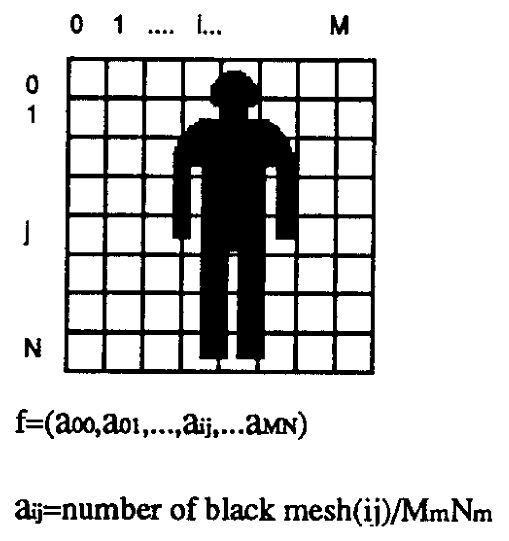
\includegraphics[width=2in]{figures/mesh-feature.jpg}  
%  \caption[Mesh feature calculation]{Mesh feature
%    calculation. Reprinted from the work of Yamato et al.\ (1992).}
%  \label{fig:mesh-feature}
%\end{figure}

%In this paper, the authors (Nair and Clark) use the coordinates of
%the blob's center of mass, average color, and height to represent a
%blob.

%Although a lot of work has tried to improve the classic background
%modeling techniques, the fragmentation problem caused by a cluttered
%background still exist in blob detection and segmentation
%process. This problem is unavoidable in practice;
%therefore, \shortciteA{lu08segmentation} attempt to solve this problem
%and propose an effective connected components labeling method called
%connected chips linking (CCL). In this paper, they provide a function
%to calculate the correlation of space location between two blobs. Then
%they construct a correlation matrix based on the result. In order to
%handle fragmented blobs, they cluster the blobs using the information
%from the correlation matrix through the mean-shift algorithm. After
%that, they classify the blob-sets into ``Human'' or ``Fragments''
%using some criteria such as human
%size. Figure \ref{fig:blob-clustering-result} shows the result of
%handling fragmented blobs.
%
%\begin{figure}[t]
%  \centering
%  \subfloat[]{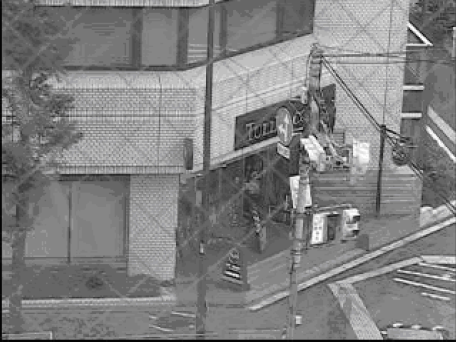
\includegraphics[scale=0.3]{figures/blob-clustering01.png}
%  \label{fig:blob-clustering01}}
%  \hspace{0.01in}
%  \subfloat[]{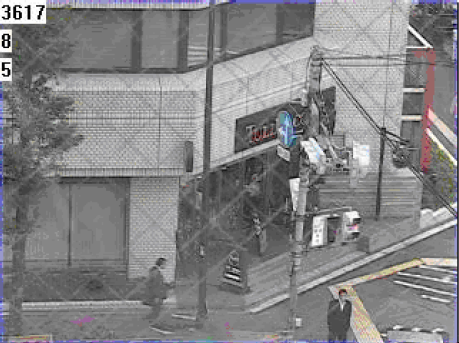
\includegraphics[scale=0.3]{figures/blob-clustering02.png}
%  \label{fig:blob-clustering02}}
%  \hspace{0.01in}
%  \subfloat[]{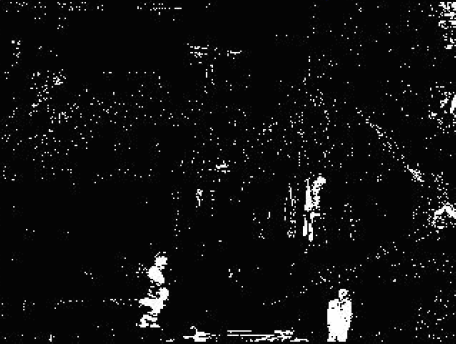
\includegraphics[scale=0.3]{figures/blob-clustering03.png}
%  \label{fig:blob-clustering03}}
%  \hspace{0.01in}
%  \subfloat[]{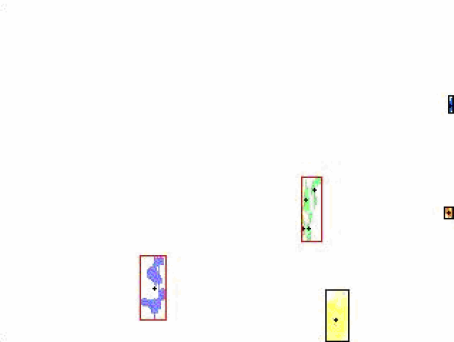
\includegraphics[scale=0.3]{figures/blob-clustering04.png}
%  \label{fig:blob-clustering04}}
%  \caption[Example of the result of handling fragmented
%  blobs.]{Example of the result of handling fragmented blobs. (a)
%  Background image. (b) Current image. (c) Foreground pixels. (d)
%  Result of handling fragmented blobs. Reprinted from the work of Lu
%  et al.\ (2008).}
%  \label{fig:blob-clustering-result}
%\end{figure}
%
%After segmenting the blob, the next step is to extract the blob
%features. \shortciteA{li06behavior} use the least median of squares
%(LMedS) method to construct the background model, then extract
%foreground by subtracting the background image. The authors propose a
%method based on space-time image features for automatic behavior
%modeling and recognition. This method is simple and insensitive to
%noise, and does not need to track parts of the human body. In this
%method, they extract the foreground, calculat shape features,
%represent the features as a space-time image. After the foreground is
%extracted, the authors equidistantly divide the bounded rectangle of
%the foreground into $10\times7$ sub-blocks. Then they normalized the
%value of each sub-block as follows:
%\[
%d_i = \left\lfloor {\frac{{s_i}}{{M}}\times255} \right\rfloor, i =
%  1,2, \ldots,k,
%\]
%where $k=10\times7$ is the number of sub-blocks; $s_i$ is the number
%of the foreground pixels in the $i^{th}$ sub-block; $M$ is the maximum
%value of $s_i$, where $i=1,2,...,k$. After that, they have the
%resulting shape descriptor $D_t$ at image frame $t$: $D_t =
%[d_1,d_2,d_3,...,d_k]$. Finally, to represent the motion of a sequence
%with $t$ frames, they construct the space time image representation
%(see Figure \ref{fig:space-time-feature}) as a matrix $I$ of size
%$t\times k$ as:
%\[
%I = [D_1,D_2,D_3,...,D_t]^{T}_{t\times k}
%\]
%They extract the features from this representation by Gabor filtering as 
%follows:
%\[
%F_n (x,y) = \iint {I_n (x_1 ,y_1 )G(x - x_1 ,y - y_1 ,f)dx_1dy_1},
%\]
%\[
%G(x,y,f) = \frac{1}{{2\pi \sigma _x \sigma _y }}\exp \left[ {
%- \frac{1}{2}\left( {\frac{{x^2 }}{{\sigma _x^2 }} + \frac{{y^2
%}}{{\sigma _y^2 }}} \right)} \right]M(x,y,f),
%\]
%\[
%M(x,y,f) = \cos \left[ {2\pi f(x\cos \theta + y\sin \theta)} \right],
%\]
%where $I_n(x,y)$ is the $n^{th}$ space-time image; $F_n(x,y)$ is the filtered 
%space-time image; the space constants of the Gaussian envelope along the $x$ 
%and $y$ axis are represented by $\delta _x$ and $\delta _y$, respectively; $f$ 
%is the frequency of the sinusoid and $\theta$ is the orientation of the Gabor 
%filter.
%
%\begin{figure}[t]
%  \centering
%  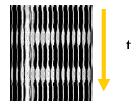
\includegraphics[width=1.5in]{figures/space-time-feature.jpg}
%  \caption[Space-time image representation]{Space-time image
%  representation. Reprinted from the work of Li et al.\ (2006)}
%  \label{fig:space-time-feature}
%\end{figure}
%
%There are some feature extraction methods that are able to capture
%motion history rather than having only current static
%features \shortcite{yamato92hmm,nair02surveillance}. One of them is
%motion history image (MHI) \shortcite{davis97mhi}. MHI is a static
%image template where pixel intensity is a function of the recency of
%motion in a video sequence. The idea is to represent how motion the
%image is moving. The MHI is defined as:
%\[
%  H_\tau  (x,y,t) = \left\{ \begin{array}{l}
%  \tau \quad \quad \quad \quad \quad \quad \quad \quad \quad \quad \quad \quad 
%  {\rm if}\;D(x,y,t) = 1 \\ 
%  \max (0,H_\tau  (x,y,t - 1) - 1)\quad {\rm otherwise}, \\ 
%  \end{array} \right.
%\]
%where $H_\tau (x,y,t)$ represents the MHI for a pixel $(x,y)$ at time
%$t$. The more recently moving pixels will be
%brighter. Figure \ref{fig:mhi} presents the examples of MHIs.
%
%\begin{figure}[t]
%  \centering
%  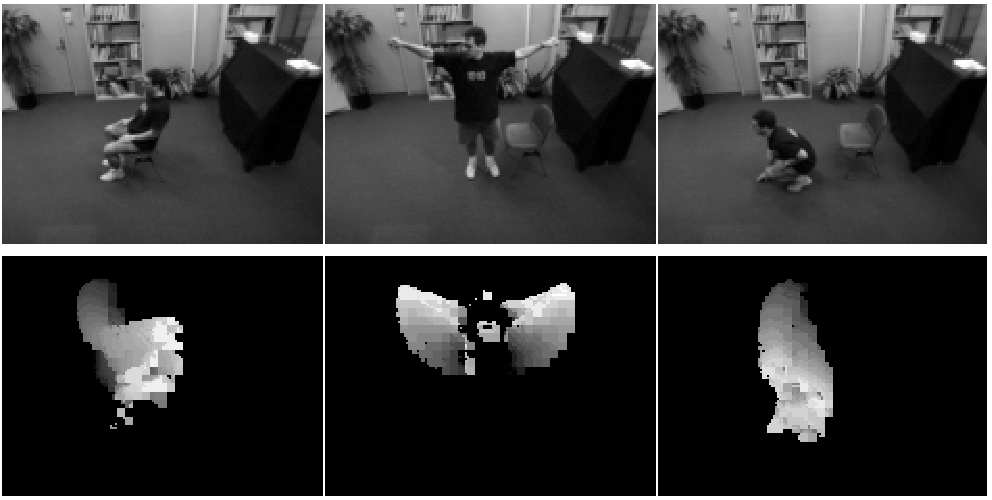
\includegraphics[width=4in]{figures/mhi}
%  \caption[Examples of motion history images]{Examples of motion
%  history images. Reprinted from the work of J. Davis \& Bobick
%  (1997).}
%  \label{fig:mhi}
%\end{figure}
%
%Based on the local intensity history of
%pixels, \shortciteA{xiang02event} proposed the pixel change history
%(PCH) to characterize pixel-wise temporal visual information in order
%to detect pixel-level events. The PCH is a representation of
%pixel-wise changes based on a combination of the pixel signal energy
%(PSE) proposed by \shortciteA{ng03pixel} and the MHI, which is
%computed as follows:
%\[
%  P_{\varsigma ,\tau } (x,y,t) = \left\{ \begin{array}{l}
%  \min (P_{\varsigma ,\tau } (x,y,t - 1) + \frac{{255}}{\varsigma },255)\quad 
%  \; {\rm if}\;D(x,y,t) = 1 \\ 
%  \max (P_{\varsigma ,\tau } (x,y,t - 1) + \frac{{255}}{\tau },0)\quad \quad 
%  {\rm otherwise}, \\ 
%  \end{array} \right.
%\]
%where $P_{\varsigma ,\tau } (x,y,t)$ represents the PCH for a pixel
%$(x,y)$ at time $t$, $D(x,y,t)$ indicates foreground regions at time
%$t$, $\varsigma$ is an accumulation factor, and $\tau$ is a decay
%factor. When the accumulation factor is set to 1, the PCH over the
%entire image is equivalent to the MHI. In this work, they did not
%specifically recognize human behaviors, but they proposed a new
%low-level primitive applicable to human representation that can
%describe human actions efficiently.
%
%Recursive filtering \shortcite{masoud03recognition} is a technique
%that encodes motion information such as the speed of the motion within
%a short period of time. The idea is to represent the ``recency'' of the
%motion. This technique is conceptually similar to the MHI. Let $I_t$
%be the frame at time $t$ and the filtered image $F_t$ at time $t$ is
%defined as follows:
%\[
%  F_t = \left| {I_t  - M_t } \right|
%\]
%\[
%  M_t = (1 - \beta)M_{t - 1}  + \beta M_t 
%\]
%\[
%  M_0 = I_0 = {\rm Background},
%\]
%where $t = 1, 2, \cdots, n_i$. If $\beta = 0$, the filtered image
%$F_t$ will be the foreground and if $\beta = 1$, $F_t$ will be
%equivalent to image differencing. Examples of filtered images are
%presented in \figurename~\ref{fig:f-img}.
%
%\begin{figure}[t]
%  \centering
%  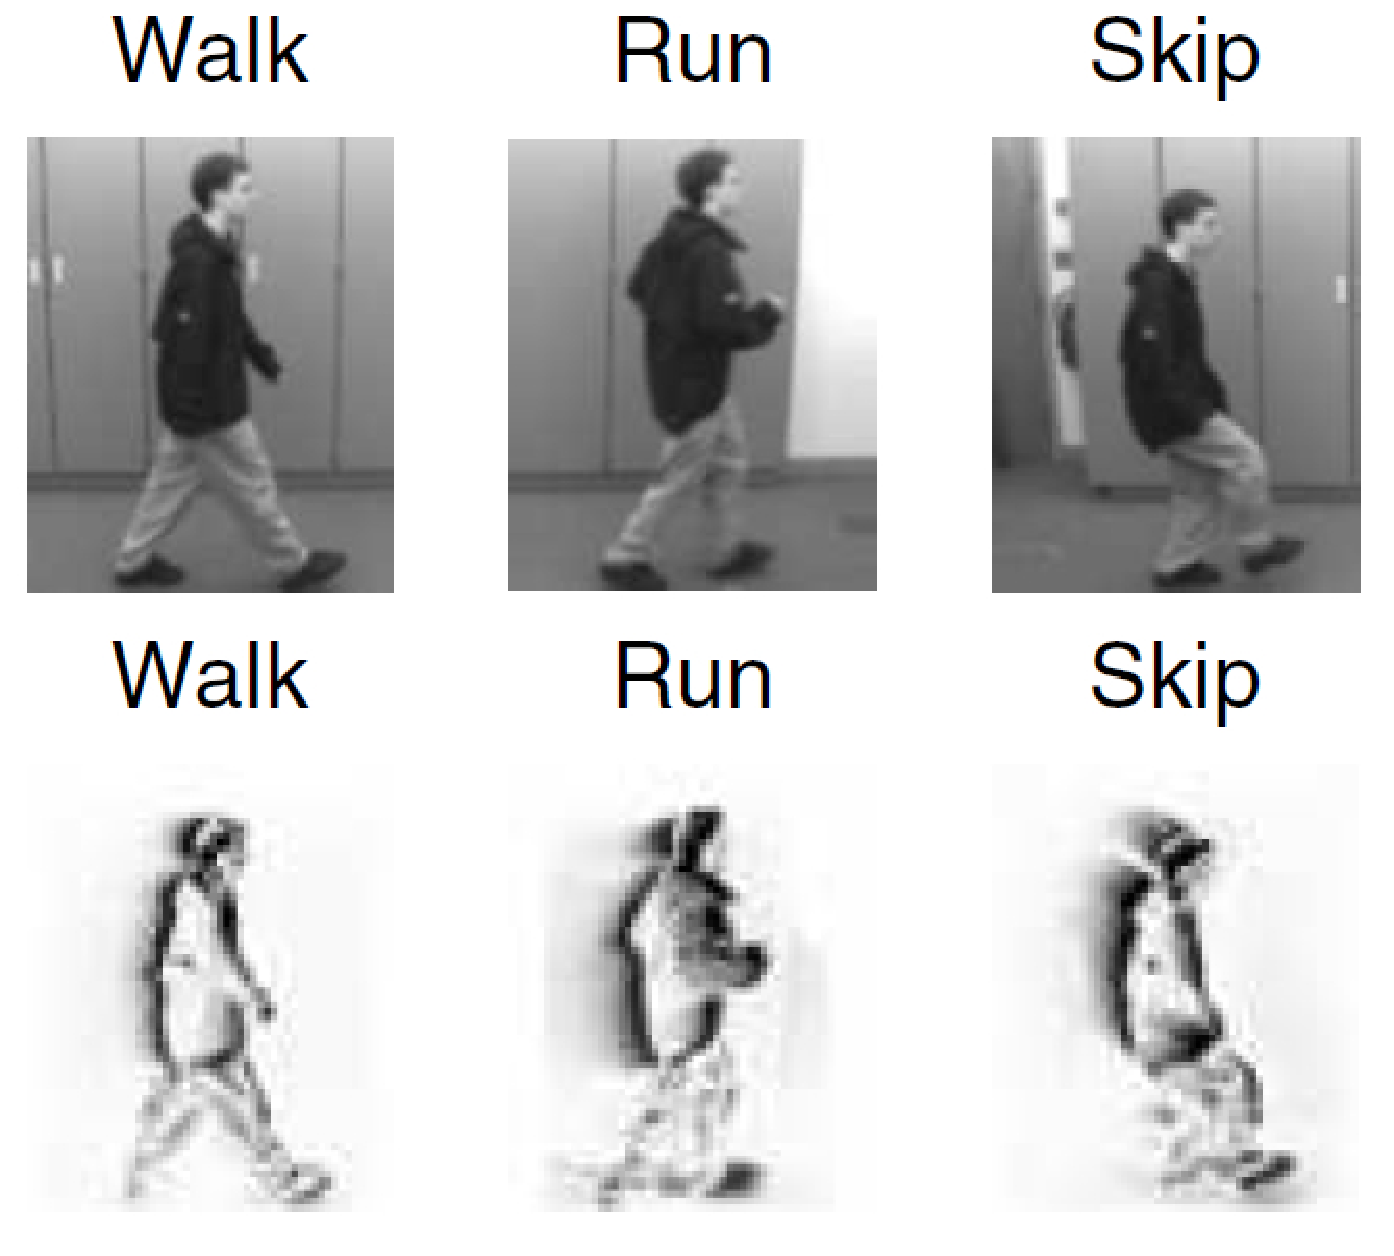
\includegraphics[width=2.5in]{figures/f-img}
%  \caption[Examples of filtered images]{Examples of filtered
%  images. The coefficient $\beta$ is set to 0.5. Reprinted from the
%  work of Masoud \& Papanikolopoulos (2003).}
%  \label{fig:f-img}
%\end{figure}
